\chapter{TÉCNICAS E PROCESSOS}

Este capítulo descreve as técnicas e os processos utilizados durante o estágio.

%A presente seção tem como objetivo citar os processos técnicos utilizados pelo estagiário durante o seu período de estágio. Ela também demonstra a fundamentação teórica onde cada etapa do estágio foi baseada.


\section{Design centrado no usuário}
O design centrado no usuário (ou UCD, do inglês \textit{User Centered Design}) é uma abordagem que visa atender às necessidades humanas, capacidades e os conhecimentos prévios dos usuários. É designado para acomodar suas necessidades, capacidades e formas de comportamento. Bons designs começam com um entendimento de psicologia e tecnologias, requerem boa comunicação, especialização da máquina para uma pessoa e indicação de quais ações são possíveis, o que está acontecendo e o que poderá acontecer. O UCD foca no entendimento das pessoas e quais são suas necessidades que o design procura encontrar, principalmente através da observação.~\cite{Norman:2002:DET:2187809} 

No design centrado ao usuário há quatro diferentes atividades:

\begin{itemize}

\item observação: uma das principais técnicas críticas é observar os possíveis usuários e o seu ambiente, independente de onde o produto será utilizado. As pesquisas de design integram essa etapa, ajudando a determinar as necessidades dos usuários;

\item geração de ideias: após o levantamento de requisitos, a segunda etapa consiste em gerar potenciais soluções;

\item prototipação;

\item testes.

\end{itemize}

\subsection{Usabilidade}

Segundo a definição abordada pela ISO 9241-11 \cite{iso9241}, a usabilidade é a eficácia, a eficiência e a satisfação que os usuários específicos têm ao atingir seus objetivos. A usabilidade pode ser compreendida como a capacidade de um sistema ser usado com facilidade pelo usuário.

Em relação à qualidade, Nielsen \cite{usabilityintroduction} afirma que a usabilidade é um atributo que avalia como as interfaces de usuário são fáceis de usar. Em relação a métodos, a usabilidade refere-se a melhoria da facilidade de utilização da interface durante o processo de concepção. Nielsen (2012) classifica a usabilidade em cinco componentes de qualidade: aprendizagem, eficiência, memorabilidade, erros e satisfação . 

A aprendizagem está relacionada a facilidade de uma tarefa ser realizada na primeira vez que o usuário se depara com o produto. A eficiência se relaciona com a rapidez que o usuário realiza suas atividades. A memorabilidade é a proficiência que o usuário terá ao retornar ao produto após algum tempo sem utilização. Os erros se relacionam na capacidade de recuperar ações indevidas dos usuários, e a satisfação está relacionada na afeição do usuário ao utilizar o produto.

Pode-se associar a usabilidade na produtividade do usuário. Se um sistema oferece uma usabilidade satisfatória, o usuário realizará suas atividades em tempo hábil e de forma prazerosa.


\subsection{Design de interação}
O design de interação está relacionado ao comportamento das pessoas em relação aos dispositivos utilizados por ela. Aspectos cognitivos e psicológicos dos usuários são registrados e estudados para se pensar em como uma interface irá se comportar junto ao usuário. O foco dos estudos do design de interação está em como as pessoas interagem com as tecnologias e em como elas manipulam. Aspectos como memória, atenção, visão e percepção podem afetar escolhas de design, e podem ser diferentes para vários tipos de usuário \cite{Norman:2002:DET:2187809}. As decisões de design são feitas no contexto do ambiente do usuário. 

O design de interação possui quatro atividades básicas: Estabelecimento de requisitos, alternativas de design, prototipação e avaliação/testes. As atividades de design de interação podem ser integradas em um modelo de processo de desenvolvimento ágil.

\section{Experiência do usuário}

No âmbito empresarial, várias empresas têm pensado qual será a experiência do usuário ao utilizar os seus produtos. A experiência do usuário (ou UX, do inglês \textit{User Experience}), além de ter a usabilidade inserida, está relacionada ao prazer que o usuário tem ao utilizar um produto. 


Segundo a definição da ISO 9241 \cite{iso9241}, a experiência do usuário está relacionada com as respostas e percepções de uma pessoa resultantes do uso de um produto, sistema ou serviço. Garret \cite{garrett2010elements} afirma que desenvolver a experiência do usuário está relacionado a assegurar que nenhum aspecto da experiência acontecerá sem a sua intenção consciente e explícita, ou seja, deve-se entender quais serão as expectativas dos usuários. 

O termo UX é, muitas vezes, utilizado de forma errônea. Muitas pessoas o utilizam apenas para focar em aspectos de interface do usuário, aplicativos e softwares. A experiência total de um produto cobre muito mais do que a sua usabilidade: estética, prazer e diversão desempenham papéis criticamente importantes. Além disso, segundo Norman \cite{NormamVideo}, a experiência é como se observa o mundo, a vida ou um serviço aspectos gerais. 



\section{Desenvolvimento ágil}
Os métodos ágeis ajudam a reduzir tempos de ciclo do desenvolvimento e entregar o valor do cliente de forma contínua. Isso significa que a entrega do software se dá de forma contínua ao cliente \cite{manifestoAgil}.

Em 2011, profissionais de software líderes da comunidade do \textit{Extreme Programming}, que possui uma abordagem orientada à objetos como paradigma de programação, e envolve atividades relacionadas a planejamento, projeto codificação e testes, declararam o Manifesto ágil \cite{agile} em quatro valores:

\begin{itemize}

\item indivíduos e interação entre eles mais que processos e ferramentas;

\item software em funcionamento mais que documentação abrangente;

\item colaboração com o cliente mais que negociação de contratos;

\item responder a mudanças mais que seguir um plano.

\end{itemize}

Após elencar os valores, foram criados os 12 princípios do manifesto ágil, que podem ser aplicados em um projeto de desenvolvimento, não se restringindo em utilizá-los em sua totalidade. Os princípios do manifesto ágil são:

\begin{enumerate}

\item nossa maior prioridade é satisfazer o cliente através de entrega prematura (antecipada) e contínua de software valioso;

\item necessidades de mudança são bem vindas, mesmo no final do desenvolvimento. Os processos Ágeis utilizam a mudança em favor da vantagem competitiva para o cliente;

\item entregar software funcionando frequentemente, com preferência em uma escala de tempo mais curto;

\item pessoas de negócios e desenvolvedores devem trabalhar juntos diariamente durante o projeto;

\item o método mais eficiente e efetivo de se transmitir informação para e entre uma equipe de desenvolvimento é a conversa face a face;

\item criar projetos em torno de indivíduos motivados. Dê-lhes o meio ambiente e apoio de que necessitam, e confiar neles para fazer o trabalho;

\item software em funcionamento é a principal medida de progresso;

\item processos ágeis promovem o desenvolvimento sustentável. Os investidores, desenvolvedores e usuários devem ser capazes de manter um ritmo constante indefinidamente;

\item atenção contínua à excelência técnica e bom design aumenta a agilidade;

\item simplicidade - a arte de maximizar a quantidade de trabalho não feito - é essencial;

\item as melhores arquiteturas, requisitos e projetos emergem de equipes auto-organizadas;

\item Em intervalos regulares, a equipe reflete e avalia sobre como se tornar mais eficaz, em seguida, ajusta seu comportamento em conformidade.

\end{enumerate}

 Atualmente, existe a Agile Aliance\footnote{https://www.agilealliance.org}, uma organização que surgiu após a declaração dos valores e princípios do Manifesto ágil, comprometida com os avanços dos princípios ágeis. 

Um dos métodos de para desenvolvimento ágil disponíveis chama-se Scrum, uma metodologia ágil para gestão e planejamento de projetos de software. Os projetos são dividos em ciclos chamados de \textit{sprints}. O \textit{sprint} representa uma faixa de tempo dentro do qual um conjunto de atividades deve ser executado \cite{scrum}. Os elementos que fazem parte de uma \textit{sprint} são:

\begin{itemize}
\item \textit{planning}: reunião de planejamento na qual o product owner lista contendo todas as funcionalidades desejadas para um produto;

\item \textit{product owner}: pessoa que define os itens que compõem o product backlog;

\item \textit{product backlog}: lista contendo todas as funcionalidades desejadas para um produto;

\item \textit{sprint backlog}: lista de tarefas que o time se compromete a fazer em um sprint.

\item \textit{daily scrum}: reunião diário que tem como objetivo disseminar conhecimento sobre o que foi feito no dia anterior, identificar impedimentos e priorizar o trabalho a ser realizado no dia que se inicia.

\item \textit{sprint review meeting}: relizada no final de cada \textit{sprint}, durante esta reunião, o time mostra o que foi alcançado durante o \textit{sprint}. 

\item \textit{sprint retrospective}: ocorre ao final de um \textit{sprint} e serve para identificar o que funcionou bem, o que pode ser melhorado e que ações serão tomadas para melhorar.

\end{itemize}

No final de cada \textit{sprint}, há a entrega do incremento de produto potencialmente viável. A metodologia ágil scrum é ilustrada na Figura \ref{fig:cicloscrum}.

\begin{figure}[H]
\centering
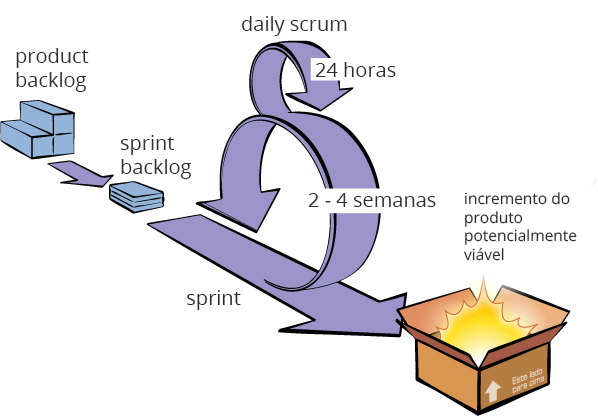
\includegraphics[width=1\textwidth]{images/ciclos_scrum.jpg}
\caption{Ciclo do Scrum. }
\label{fig:cicloscrum}
{\small Fonte: http://www.desenvolvimentoagil.com.br/scrum. Acessado em: 01/02/2017} %Fonte da imagem
\end{figure}


%TODO completar a frase (done!)

O método mais eficiente e eficaz de transmitir informação para e dentro de uma equipe de desenvolvimento é a conversa face-a-face. Tratando-se da experiência do usuário, surgiu o conceito de \textit{Lean UX}, que é o desenvolvimento ágil focado no usuário.

O \textit{Lean UX} é definido como uma abordagem para um desenvolvimento de software centrado no usuário, especialmente em \textit{startups}, criando produtos radicalmente novos. Ele tenta romper com os silos organizacionais e ciclos de produção como, por exemplo, o processo de desenvolvimento de software em cascata \cite{Liikkanen:2014:LUN:2639189.2670285}. 

São identificadas três principais influências no \textit{Lean UX}: movimento \textit{design thinking}, método \textit{Learn startup} e desenvolvimento de software ágil \cite{gothelf2013lean}.

O \textit{design thinking} é importante para o \textit{Lean UX} pois toma a posição explícita de que todos os aspectos de um negócio podem ser abordados com métodos de design. O pensamento de design é uma fundação crítica que incentiva as equipes a colaborar entre papéis e considerar o design do produto de uma perspectiva holística \cite{robbinsd:beck2001agile}.

A \textit{Lean Startup} defende a criação de protótipos rápidos projetados para testar as premissas do mercado e usa o \textit{feedback} dos clientes para evoluí-los muito mais rápido do que as práticas de engenharia de software tradicionais \cite{robbinsd:beck2001agile}. Esse método aumenta a frequência de contato com os clientes e minimizam o risco de entregas atrasadas do projeto e faz com que a equipe desenvolva mais rapidamente.

\section{Desenvolvimento front-end}
O desenvolvimento \textit{front-end} está relacionado a aspectos visuais e é onde o usuário interage com a aplicação diretamente, para que o \textit{back-end} - linguagens de programação - possa processar esses dados. Durante o desenvolvimento \textit{front-end}, muito se foi pensando na responsividade das páginas.

O web design responsivo é uma abordagem de desenvolvimento web que cria alterações dinâmicas na aparência de um site, dependendo do tamanho da tela e da orientação do dispositivo usado para visualizá-lo \cite{ResponsiveWebDesignNNG}.

Com a utilização de padrões web como HTML5, CSS e Javascript, ou do \textit{framework} Bootstrap, é possível desenvolver páginas web responsivas que podem adaptar a arquitetura da informação de uma página em qualquer tamanho e resolução de tela.

Por meio de um layout fluido, conteúdo flexível e de padrões web que podem  detectar capacidades de tamanho de tela, resolução, densidade de pixel e orientação, desenvolvedores podem criar contextos e adaptáveis \cite{Responsive}.

O HTML (Linguagem de Marcação de Hypertexto, do inglês HyperText Markup Language) é uma linguagem que descreve o conteúdo de documentos web \cite{html5}. Na sua versão 5, possui características que tornam fáceis o trabalho com multimídias e gráfica, sem recorrer a plugins e APIs de terceiros.

O CSS (Folha de estilo em cascata, do inglês \textit{Cascate Style Sheet}) é uma linguagem que descreve o estilo de um documento HTML. O CSS, atualmente na versão 3, formata a informação entregue pelo HTML. Essa informação pode ser imagem, fontes, texto, vídeo, áudio ou qualquer outro elemento criado \cite{css3}. Ele permite adaptar a apresentação da informação em diferentes tipos de dispositivos, com tamanhos diferentes de telas e também auxilia na formatação de informações para impressão.

O Javascript (Js) é uma linguagem de programação interpretada de múltiplos paradigmas,
baseado na orientação a objetos, imperativo e declarativo \cite{javascript}. Já o Bootstrap, um \textit{framework} de código livre para desenvolvimento de projetos responsivos, que se adaptam à diferentes resoluções de tela, baseado em Javascript, assim como em HTML5 e CSS3.


\section{Análise e especificação de requisitos}

Requisito é uma afirmação sobre um produto a ser projetado, que especifica o que deve, o que não deve, ou como deve ser construído \cite{Sommerville:2010:SE:1841764}. Um dos principais objetivos do estabelecimento de requisitos é fazê-los específicos e claros. A ampla área de tarefas e técnicas que levam à compreensão dos requisitos é chamado de. engenharia de requisitos. 

A engenharia de requisitos é uma ação de engenharia de software que começa durante a atividade de comunicação e continua na atividade de modelagem. Deve ser adaptada as necessidades do processo, do projeto, do produto e das pessoas que fazem o trabalho \cite{Pressman:2001:SEP:572512}. 


\section{Prototipação}

Uma das formas mais eficazes de criar um MVP é através da prototipagem de experiência do usuário. Um protótipo é uma aproximação de uma experiência que permite simular o que é e como usar o produto ou serviço em questão necessitando, então, de ser clicável. Ao mesmo tempo, seu objetivo deve ser gastar o menor esforço possível para criar o protótipo, o que torna a escolha da ferramenta de prototipagem importante. No processo da engenharia de requisitos, o protótipo pode ajudar na elicitação e validação dos requisitos \cite{Sommerville:2010:SE:1841764}.

O \textit{wireframe} é uma representação de baixa fidelidade de uma interface. Mockup é uma representação estática de média a alta fidelidade, e protótipo é uma representação dinâmica de alta fidelidade, simulando a interface de interação com o usuário \cite{Sommerville:2010:SE:1841764}.

\subsection{Protótipo de baixa fidelidade}

Os protótipos de baixa fidelidade podem ser feitos dos componentes mais acessíveis como papel, canetas, permitindo simular experiências de uma maneira rápida. Nenhum investimento é necessário e permite a equipe um senso de como o produto deve funcionar \cite{Sommerville:2010:SE:1841764}.

\subsection{Protótipo de alta fidelidade}
Os protótipos de alta e média fidelidade têm significativamente mais detalhes do que os protótipos baseados em \textit{wireframes}. Pode-se utilizá-los para demonstrar e testar projetos que são desenvolvidos com um nível de interação semelhante da experiência do produto final \cite{Sommerville:2010:SE:1841764}.


\section{Avaliação Heurística}
% TODO - é importante descrever aqui o que é uma avaliação heurística, como é feita, em termos conceituais, já que você utilizou no projeto (done!)

A avaliação heurística é um método informal para a análise da usabilidade e é realizada inspecionando uma interface, e tentando chegar a uma opinião sobre o que é bom e ruim sobre ela. Tem como vantagem ser barata, intuitiva e fácil de motivar as pessoas a fazê-la. Ela não requer um planejamento avançado, e pode ser usado claramente no desenvolvimento de processos. Como desvantagem, este método, às vezes, identifica problemas de usabilidade sem prover sugestões diretas em como resolvê-los ~\cite{Nielsen:1990:HEU:97243.97281}.

Ela tem como objetivo encontrar problemas de usabilidade em designs de interface de usuário, com um pequeno número de avaliadores que examinam e julgam uma interface e suas complicações, com base nos princípios de usabilidade \cite{Nielsen:1992:FUP:142750.142834}.


Cada participante classifica o problema a um fator de gravidade de acordo com as severidades propostas por \cite{severidades}, considerando a influência dos problemas na realização das atividades. A classificação das severidades ajudam a fornecer uma estimativa aproximada da necessidade de esforços adicionais de usabilidade. As cinco severidades são:

  
0 = Não acredito que seja um problema

1 = Cosmético: Não há necessidade imediata de solução

2 = Pequeno: Problema de baixa prioridade

3 = Grande: Problema de alta prioridade

4 = Catástrofe: Problema muito grave, deve ser reparado imediatamente


Na avaliação heurística colaborativa, cada participante é livre para indicar um problema na interface.  Ao final da avaliação, para catalogar os dados, foi realizada uma média das severidades dada pelos 5 especialistas participantes à cada problema, e atribuído, a cada um, sua(s) heurística(s) correspondente(s), segundo as 10 heurísticas propostas por Nielsen e Molich \cite{Nielsen:1990:HEU:97243.97281}:


Heurística 1 - Visibilidade do status do sistema: O sistema deve sempre manter os usuários informados sobre o que está acontecendo, através de feedback adequado dentro de um prazo razoável.

Heurística 2 - Correspondência entre o sistema e o mundo real: O sistema deve falar o idioma dos usuários, com palavras, frases e conceitos familiares para o usuário, em vez de termos orientados ao sistema. Siga as convenções do mundo real, fazendo com que as informações apareçam em uma ordem natural e lógica.


Heurística 3 - Controle do usuário e liberdade: Os usuários muitas vezes escolhem funções do sistema por engano e precisarão de uma "saída de emergência" claramente marcada para deixar o estado indesejado sem ter que passar por um diálogo estendido. Suporte desfazer e refazer.

Heurística 4 -  Consistência e padrões: Os usuários não devem ter que se perguntar se diferentes palavras, situações ou ações significam a mesma coisa. Siga as convenções da plataforma.

Heurística 5 - Prevenção de erros: Melhor do que boas mensagens de erro é um design cuidadoso que impede que um problema ocorra em primeiro lugar. Elimine as condições propensas a erros ou procure por elas, e apresente aos usuários uma opção de confirmação antes de se comprometerem com a ação.

Heurística 6 - Reconhecimento em vez de recordação: Minimize a carga de memória do usuário, tornando visíveis objetos, ações e opções. O usuário não deve se lembrar de informações de uma parte do diálogo para outra. As instruções de utilização do sistema devem ser visíveis ou facilmente recuperáveis sempre que adequado.        

Heurística 7 - Flexibilidade e eficiência de utilização: Aceleradores - invisível pelo usuário novato - muitas vezes pode acelerar a interação para o usuário especializado, de tal forma que o sistema pode servir tanto para usuários inexperientes e experientes. Permita que os usuários adaptem ações frequentes.  

Heurística 8 -  Estética e design minimalista: Os diálogos não devem conter informações irrelevantes ou raramente necessárias. Cada unidade extra de informação em um diálogo compete com as unidades relevantes de informação e diminui sua visibilidade relativa.     


Heurística 9 - Ajude os usuários a reconhecer, diagnosticar e resolver erros:  Mensagens de erros devem ser expressas em linguagem clara (sem códigos), indicar com precisão o problema e construtivamente sugerir uma solução.

Heurística 10 - Ajuda e documentação: Mesmo que seja melhor que um sistema pudesse ser usado sem documentação, pode ser necessário fornecer uma ajuda e documentação. Qualquer informação deve ser fácil de ser pesquisada, com foco na atividade do usuário, lista de passos concretos a serem realizados, e não ser muito grande.   



